\documentclass[notheorems, handout]{beamer}

\usetheme{Warsaw}
\setbeamertemplate{page number in head/foot}[totalframenumber]
\setbeamertemplate{headline}{}
\setbeamertemplate{navigation symbols}{}
\usefonttheme[onlymath]{serif}

\usepackage[utf8]{inputenc}
\usepackage[T2A]{fontenc}
\usepackage[russian]{babel}

\usepackage{graphicx,subcaption,ragged2e}
\usepackage{tikz}
\usepackage{bm}

\newtheorem{remark}{Замечание}

\title[Статистическое и машинное обучение]{Обучение с учителем}
\institute[Санкт-Петербургский Государственный Университет]{%
	\small
	Санкт-Петербургский государственный университет\\
	Кафедра статистического моделирования
}
\date{16 сентября 2025, Санкт-Петербург}

\begin{document}

\begin{frame}
	\titlepage
\end{frame}

\begin{frame}{Введение}
	\textbf{Машинное обучение}~--- это раздел искусственного интеллекта, в котором разрабатываются методы и алгоритмы, позволяющие компьютерам обнаруживать закономерности в данных и делать прогнозы без явных инструкций.\medskip

	\textbf{Обучение с учителем}~--- один из способов машинного обучения, в ходе которого для каждого примера в обучающем наборе известно, какой результат является правильным.\medskip

	\textbf{Пример задач}:
	\begin{itemize}
		\item Регрессия: предсказание стоимости недвижимости, количества продаж некоторого товара, погоды.
		\item Классификация: предсказание ценовой категории товара, типа изображения, болеет ли человек или нет.
	\end{itemize}
\end{frame}

\begin{frame}{Постановка задачи}
	\textbf{Дано}:
	\begin{enumerate}
		\item Пространство объектов $X$~--- множество описаний объектов (например, фотографии, тексты, таблицы с признаками).
		\item Пространство ответов $Y$~--- множество меток или значений, которые нужно предсказывать (например, классы <<кот>>/<<собака>>, цена товара).
		\item Обучающая выборка $D = \{(x_i, y_i)\}_{i=1}^n$, где $x_i\in X$, $y_i\in Y$.
	\end{enumerate}
	\textbf{Модель}:
	\[
		y=f(x) + \varepsilon,
	\]
	где $f(x)$~--- некоторая фиксированная (но неизвестная) функция, $\varepsilon$~--- шум, $\mathsf{E}\varepsilon=0$ и $\varepsilon$ не зависит от $x$.\medskip
	% \]
	% \[
	% a:X\longrightarrow Y,
	% \]
	% сопоставляющая набору признаков значение целевой переменной.\medskip

	\textbf{Предположение}: $f(x)$ лежит в некотором классе функций (например, в классе линейных функций).\medskip

	\textbf{Задача}: по обучающей выборке $D$ построить оценку $\hat f(x)$ функции $f(x)$ в выбранном классе функций.
	% чтобы ее предсказания $\hat y=\hat a(x)$ были как можно ближе к истинным ответам $y$.
\end{frame}

\begin{frame}{Функция потерь и ее минимизация}
	Чтобы оценить, насколько хорошо модель предсказывает ответы, используется {\bf функция потерь} $L(y, \hat{y})$. Она показывает, насколько велико расхождение между истинными значениями $y$ и его предсказаниями $\hat{y}$.\bigskip

	Тогда задача машинного обучения~--- минимизация выбранной функции потерь:
	\[
		L(y, \hat y)\longrightarrow \min.
	\]\smallskip

	В большинстве случаев вычислить точку минимума функции потерь аналитически не представляется возможным, поэтому для его нахождения прибегают к методам \textbf{детерменированной и стохастической оптимизации} (например, перебор значений по сетке, метод Ньютона и квазиньютоновские методы, (стохастический) градиентный спуск, случайный поиск).

	% {\bf Примеры}:
	% \begin{itemize}
	% 	\item Для задачи \textbf{регрессии} наиболее распространенной функцией потерь является среднеквадратичная ошибка (MSE):
	% 	      \[
	% 		      L(y, \hat{y}) = \frac{1}{n}\sum_{i=1}^n (y_i - \hat y_i)^2.
	% 	      \]
	% 	\item Для задачи \textbf{бинарной классификации}, если $\hat y$ представляет собой вектор вероятностей принадлежности к положительному классу, используется кросс-энтропия:
	% 	      \[
	% 		      L(y, \hat{y}) = -\sum_{i=1}^n\left[y_i \ln\hat y_i + (1 - y_i)\ln (1 - \hat y_i)\right].
	% 	      \]
	% \end{itemize}
\end{frame}

\begin{frame}{Градиентный спуск}
	Градиентный спуск является наиболее распространенным алгоритмом оптимизации в машинном обучении.\medskip

	Пусть $f$~--- некоторая гладкая функция, у которой необходимо найти минимум. Обозначим $p_n=-\nabla f(x_n)$~--- направление антиградиента в точке $x_n$. Тогда
	\[
		x_{n+1}=x_n+\alpha p_n,
	\]
	где $\alpha$~--- гиперпараметр, отвечающий за скорость обучения.\medskip

	\textbf{Условия сходимости}: выпуклость $f$, липшицевость $\nabla f$, ...\medskip

	\textbf{Критерий остановки}: достижение определенного числа итераций, малая норма градиента, малое изменение значения функции.
\end{frame}

\begin{frame}{Модификации градиентного спуска}
	В машинном обучении:
	\[
		f(x)=\frac{1}{n}\sum_{i=1}^n f_i(x),
	\]
	где $f_i$~--- функция потерь для $i$-го наблюдения.\medskip
	\begin{enumerate}
		\item (Batch) Gradient Descent (GD):
		      \[
			      p_n=-\nabla f(x_n)=-\sum_{i=1}^n \nabla f_i(x_n).
		      \]
		\item Mini-batch GD: случайным образом выбирается \textsf{m} наблюдений и делается шаг с $p_n=-\sum_{i=1}^m \nabla f_{j_i}(x_n)$.\smallskip
		\item Stochastic GD: mini-batch GD с $m=1$.\smallskip
		\item Adam (Adaptive Moment Estimation): основан на GD, каждый параметр модели имеет собственную адаптивную скорость обучения, основанную на прошлых градиентах.
	\end{enumerate}
\end{frame}

\begin{frame}{Процесс обучения}
	Процесс обучения любого алгоритма машинного обучения выглядит следующим образом:
	\begin{enumerate}
		\item Выборка $D$ предварительно разбивается на тренировочную и тестовую: $D=D_\text{train} \sqcup D_\text{test}$ .\medskip
		\item На тренировочных данных модель обучается: минимизируется выбранная функция потерь $L(y, \hat y)$.\medskip
		\item Также часто присутствует и валидационная выборка $D_\text{val}$, на основе которой подбираются гиперпараметры модели/производится остановка оптимизации функции потерь.
	\end{enumerate}
\end{frame}

\begin{frame}{Оценка качества модели}
	После обучения нужно оценить качество/обобщающую способность модели. Для этого на тестовом множестве вычисляются различные метрики. Выбираются они в зависимости от задачи.\smallskip

	Важно понимать разницу между функцией потерь и метрикой качества:
	\begin{itemize}
		\item Функция потерь возникает в тот момент, когда мы сводим задачу построения модели к задаче оптимизации.
		\item Метрика — внешний, объективный критерий качества, обычно зависящий не от параметров модели, а только от предсказанных меток.
	\end{itemize}
	\begin{table}[h!]
		\centering
		\caption{Метрики для задач регрессии и классификации}
		\begin{tabular}{|p{3cm}|p{6cm}|}
			\hline
			Регрессия & MSE, RMSE, MAE, MAPE, WAPE \\
			\hline
			Классификация & Accuracy, Precision, Recall, F1-score, ROC AUC, PR AUC \\
			\hline
		\end{tabular}
	\end{table}\medskip
\end{frame}

\begin{frame}{Линейная классификация}
	Пусть целевая переменная $y$ принимает значения $\{-1, 1\}$. Хотим обучить линейную модель так, чтобы плоскость, которую она задает, как можно лучше отделяла объекты одного класса от другого.\medskip

	Линейный классификатор:
	\[
		\hat y = \hat f(x; w) = \operatorname{sign} \langle x, w\rangle.
	\]
	Функция потерь:
	\[
		L(y, \hat{y}) = \sum_{i=1}^{n}\mathbb{I}[y_i \langle x_i, w\rangle < 0] \longrightarrow \min_{w}.
	\]
\end{frame}

\begin{frame}{Линейная классификация. Отступ}
	Величина $M_i=y_i \langle x_i, w\rangle$ называется \textbf{отступом} (margin) классификатора. Абсолютная величина отступа говорит о степени уверенности классификатора.\medskip

	\textbf{Проблема}: функция $\mathbb{I}[M < 0]$ кусочно-постоянная, следовательно функцию потерь невозможно оптимизировать градиентными методами, поскольку во всех точках производная равна нулю.\medskip

	\textbf{Решение}: можно мажорировать эту функцию более гладкой функцией и минимизировать функцию потерь с этой мажорирующей функцией с помощью методов численной оптимизации.
\end{frame}

\begin{frame}{Линейная классификация. Функции потерь}
	\begin{enumerate}
		\item Перцептрон: $L(M) = \max(0, -M)$~--- отступы учитываются только для неправильно классифицированных объектах пропорционально величине отступа.
		\item Hinge (SVM): $L(M) = \max(0, 1-M)$~--- объекты, которые классифицированы правильно, но не очень <<уверенно>>, продолжают вносить свой вклад в градиент.
		\item Логистическая: $L(M) = \ln\left(1+e^{-M}\right)$.
	\end{enumerate}
	\begin{figure}
		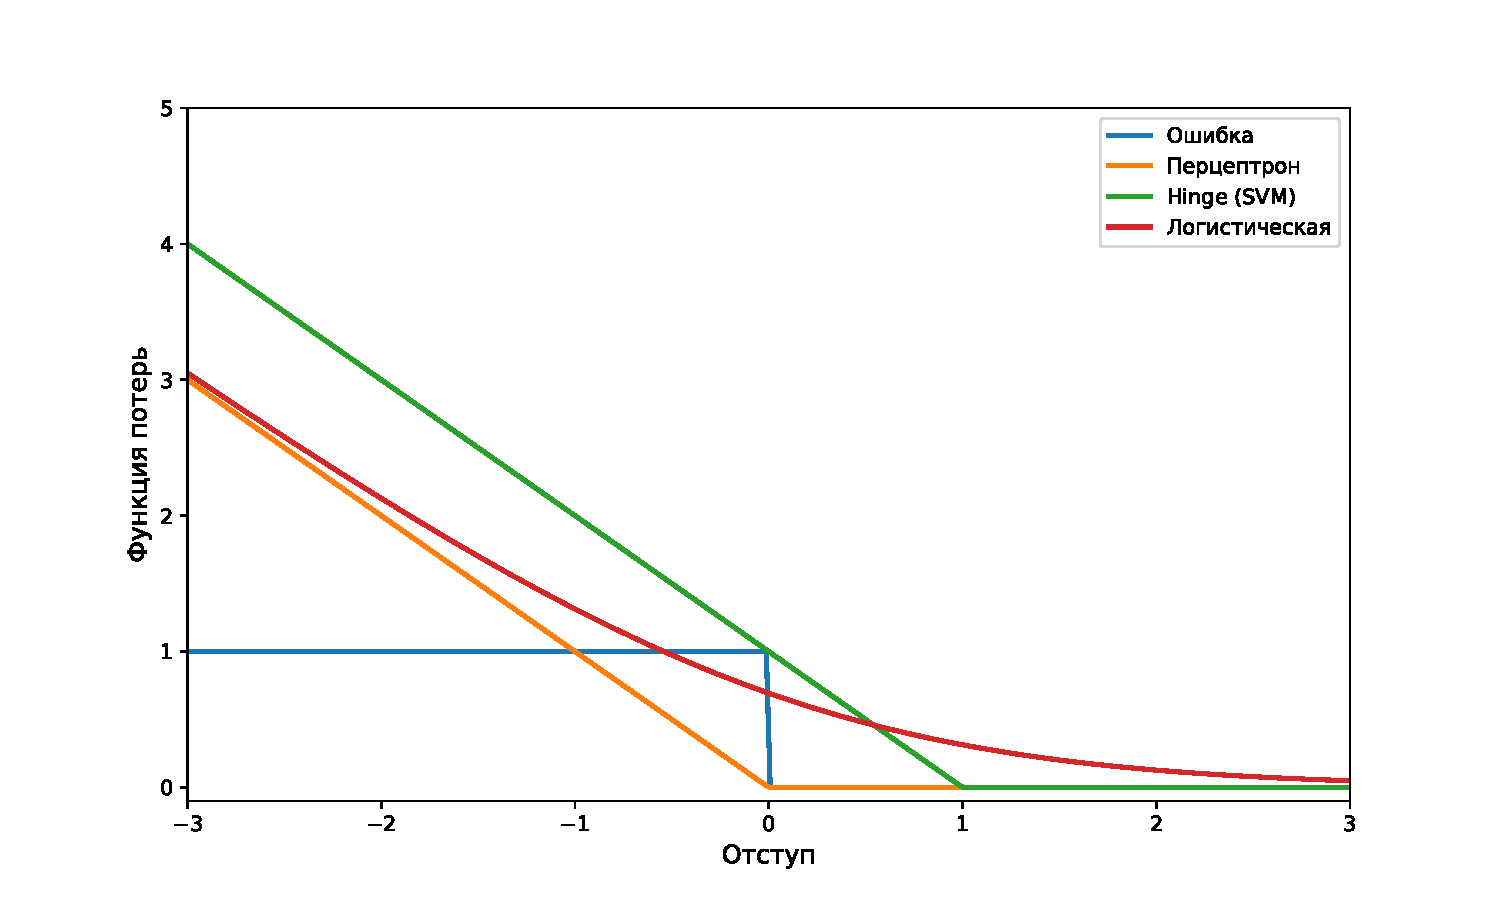
\includegraphics[width=0.75\textwidth]{img/loss_major.pdf}
	\end{figure}
\end{frame}

\begin{frame}{Логистическая регрессия}
	Посмотрим на задачу классификации как на задачу предсказания вероятностей (например, предсказание <<кликабельности>> рекламного баннера).

	\textbf{Принцип работы}: научить линейную модель предсказывать значения $z\in\mathbb{R}$ (логиты), а затем преобразовывать их в вероятности с помощью сигмоиды:
	\[
		z_i=\langle x_i, w\rangle = \ln\frac{p_i}{1 - p_i},\quad p_i = \frac{1}{1+e^{-\langle x_i, w\rangle}}=\sigma(\langle x_i, w\rangle).
	\]
	Функция правдоподобия для распределения Бернулли:
	\[
		p(y~|~\mathbf{X}, w)=\prod_{i=1}^np_i^{y_i}(1-p_i)^{1-y_i}.
	\]
	Прологарифмируем:
	\[
		\sum_{i=1}^n\Big[y_i\ln(\sigma(\langle x_i, w\rangle)) + (1-y_i)\ln(1-\sigma(\langle x_i, w\rangle))\Big].
	\]
\end{frame}

\begin{frame}{Логистическая регрессия. Связь с отступом}
	Теперь пусть $y\in\{-1, 1\}$. Тогда, поскольку $\sigma(z)=1-\sigma(-z)$, логарифм правдоподобия можно представить в следующем виде:
	\begin{align*}
		\ln p (y~|~ \mathbf{X}, w) & = -\sum_{i=1}^n\Big[\mathbb{I}[y_i=1]\sigma(z_i)+\mathbb{I}[y_i=-1]\left(1-\sigma(z_i)\right)\Big] \\
		                           & = -\sum_{i=1}^n \ln\sigma(y_i\langle x_i, w\rangle)                                                \\
		                           & = \sum_{i=1}^n \ln\left(1 + e^{-M}\right)
	\end{align*}

	Таким образом, функцию потерь в логистической регрессии можно представить в виде функции от отступа.
\end{frame}

\end{document}